\chapter{Foglio \ \thechapter}


\section*{Quesito 1}
\addcontentsline{toc}{section}{Quesito 1}
Dare le definizioni di: curva, equazioni parametriche di una curva, sostegno
di una curva, curva semplice, curva chiusa. Esibire: una curva semplice, una curva che
non è semplice, una curva chiusa, una curva che non è chiusa, due curve diverse con lo
stesso sostegno.

\medskip
\begin{large}
\textbf{Soluzione}
\end{large} \\
%==== Curva, Equazioni e Sostegno =====================================================
Si dice \textbf{Curva} un'applicazione continua $\varphi : I\subseteq \R\to\R^n$
e chiamiamo \textbf{Equazioni Parametriche} le equazioni:
\[
  t\in I \quad \varphi(t)=\left\{\begin{array}{l}
      x_1=\varphi_1(t)\\
      \vdots\\
      x_n=\varphi_n(t)
  \end{array}\right.  
\]
Inoltre definiamo \textbf{Sostegno} della Curva l'insieme $\varphi(I)\subseteq\R^n$\\
%==== Semplici, Chiusa =====================================================
Diremo che una Curva $\varphi: I\to\R^n$ è \textbf{Semplice} se:
\[
\forall t_1,t_2\in I \text{ con } t_1\neq t_2 \text{ (di cui uno interno) } \implies \varphi(t_1)\neq\varphi(t_2)  
\]
Una curva $\varphi:[a,b]\to\R^n$ invece si dice \textbf{Chiusa} se $\varphi(a)=\varphi(b)$.\\
%==== Esempi =================================================
\smallskip
\textbf{Esempi:}
\begin{align*}
  &\text{ Semplice: } \gamma(t)=(\cos t, \sin t)\: t\in[0,2\pi]\\
  &\text{ Non Semplice: } \gamma(t)=(\cos t, \sin t)\: t\in[0,4\pi]\\
  &\text{ Chiusa: } \gamma(t)=(\cos t, \sin t)\: t\in[0,2\pi]\\
  &\text{ Non Chiusa: } \gamma(t)=(t^2, t)\: t\in[0,1]\\
  &\text{ Curve diverse con stesso sostegno: } \gamma(t)=(\cos t, \sin t)\: t\in[0,2\pi] \text{ e }\gamma(t)=(\cos t, \sin t)\: t\in[0,4\pi]
\end{align*}


\section*{Quesito 2}
\addcontentsline{toc}{section}{Quesito 2}
Dare le definizioni di curva regolare, di curva regolare a tratti, di versore
tangente $T$. Esibire una curva di classe $C^1$
il cui sostegno abbia una cuspide.


\medskip
\begin{large}
\textbf{Soluzione}
\end{large}\\
Diremo che una Curva $\varphi : I = [a,b]\subseteq \R\to\R^n$ è \textbf{Regolare}
se:
\[
  \varphi\in C^1(I) \text{ e } \forall t \in (a,b) \quad \varphi'(t)\neq 0
\text{ (o equivalentemente } \|\varphi'(t)\|^2\neq0).
\]
Diremo invece che è \textbf{Regolare a Tratti}
se l'insieme I è divisibile in N ($\in\N$) tratti
in cui $\varphi$ è Regolare. Infine chiamiamo \textbf{Versore Tangente}
alla Curva nel punto $t_0$ il vettore:
\[
T(t_0)=\frac{\varphi'(t_0)}{\|\varphi'(t_0)\|}  
\]
Un esempio di Curva $C^1$ con Cuspide è il seguente:
\[
\varphi(t)=(t^3,t^2)\quad t\in[-1,1]
\]
Infatti si nota facilmente che $\varphi\in C^1([-1,1])$,
tuttavia non è Regolare in $0$ poichè $\varphi'(0)=(0,0)$. Se ne facciamo il grafico:
\begin{figure}[h]
  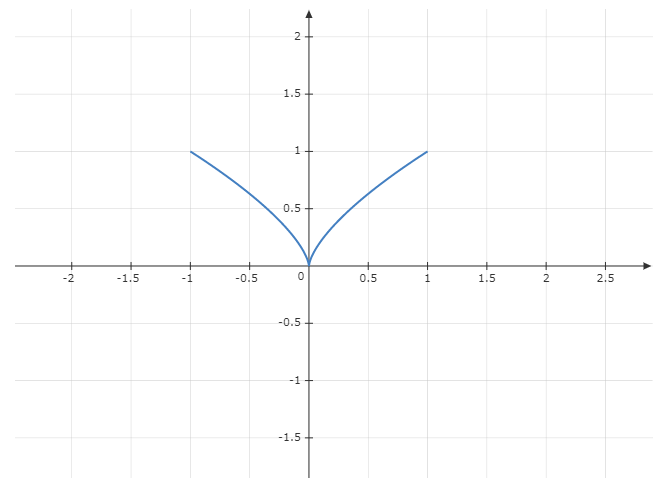
\includegraphics[width=\textwidth]{cuspide.png}
\end{figure}


\section*{Quesito 3}
\addcontentsline{toc}{section}{Quesito 3}
Dire cosa si intende per orientamento o verso di percorrenza di una curva.
Esibire due curve con lo stesso sostegno, ma con orientamento opposto. Dare la definizione
di curve equivalenti. Sotto quali condizioni sul cambiamento di parametro due curve
equivalenti hanno lo stesso orientamento o orientamento opposto?


\medskip
\begin{large}
\textbf{Soluzione}
\end{large}\\
Diremo che un punto $P_1=\varphi(t_1)$ di una Curva precede un altro punto $P_2=\varphi(t_2)$ se $t_1<t_2$.
Due curve con stesso sostegno ma orientamento opposto sono le seguenti:
\[
\varphi(t)=(\cos t, \sin t) \text{ e } \gamma(t)=(\sin t, \cos t) \text{ con } t\in [0,2\pi]  
\]
Diremo che due Curve $\varphi:I\to\R^n$ e $\gamma:J\to\R^n$ sono \textbf{Equivalenti} se:
\[
\exists \: g:I\to J \text{ suriettiva},\:C^1,\:g'(t)\neq0\;\forall t\in I \text{ tale che: } \varphi(t)=\gamma(g(t))
\]
E inoltre avranno lo stesso verso se $g'(t)>0$ e opposto se invece $g'(t)<0$
\section*{Quesito 4}
\addcontentsline{toc}{section}{Quesito 4}
Dare le definizioni di lunghezza di una curva e di curva rettificabile. Scrivere
la formula che fornisce la lunghezza di una curva di classe $C^1$.


\medskip
\begin{large}
\textbf{Soluzione}
\end{large}\\



\section*{Quesito 5}
\addcontentsline{toc}{section}{Quesito 5}
Cosa si intende per ascissa curvilinea (o parametro d’arco). Mostrare che data
una curva regolare si può sempre trovare una curva ad essa equivalente parametrizzata
con l’ascissa curvilinea.


\medskip
\begin{large}
\textbf{Soluzione}
\end{large}


\section*{Quesito 6}
\addcontentsline{toc}{section}{Quesito 6}
Scrivere la definizione di integrale curvilineo di prima specie. Dimostrare che
l’integrale curvilineo di prima specie è invariante per curve equivalenti. Dedurne che due
curve equivalenti hanno la stessa lunghezza.

\medskip
\begin{large}
\textbf{Soluzione}
\end{large}


\section*{Quesito 7}
\addcontentsline{toc}{section}{Quesito 7}
Sia $\varphi = \varphi(s)$ una curva con $s$ ascissa 
curvilinea. Dare la definizione di curvatura di $\varphi$ e 
spiegarne il significato geometrico. Quando $\varphi$ si dice 
biregolare? Riferendosi a $\varphi$, dare le definizioni di: 
versore normale principale $N(s)$, versore binormale $B(s)$.
Mostrare che $T(s)$, $N(s)$, $B(s)$ formano una base
 ortonormale di $\R ^3$
. Scrivere le definizioni
dei piani osculatore, normale, rettificante. Dire cosa si intende per cerchio osculatore e
per raggio di curvatura.


\medskip
\begin{large}
\textbf{Soluzione}
\end{large}


\section*{Quesito 8}
\addcontentsline{toc}{section}{Quesito 8}
Dare la definizione di curva piana. Sia $\varphi = \varphi(s)$ una
 curva con $s$ ascissa
curvilinea. Definire la torsione di $\varphi$ e illustrarne il 
significato geometrico. In che modo la
torsione e il versore binormale sono collegati al fatto che 
una curva è piana?

\medskip
\begin{large}
\textbf{Soluzione}
\end{large}


\section*{Quesito 9}
\addcontentsline{toc}{section}{Quesito 9}
Scrivere e dimostrare le formule di Frénet.

\medskip
\begin{large}
\textbf{Soluzione}
\end{large}


\section*{Quesito 10}
\addcontentsline{toc}{section}{Quesito 10}
Data una curva $\varphi = \varphi(t)$ con $t$ parametro qualsiasi, 
scrivere $T(t)$, $N(t)$, $B(t)$,
la curvatura $\kappa(t)$ e la torsione $\tau (t)$. Inoltre, 
scrivere e dimostrare la formula di decomposizione dell’accelerazione.

\medskip
\begin{large}
\textbf{Soluzione}
\end{large}
